\documentclass[11pt]{article}

\usepackage[margin=1in]{geometry}
\usepackage{amssymb, amsthm, amsmath}
\makeatletter
\renewcommand*\env@matrix[1][*\c@MaxMatrixCols c]{%
  \hskip -\arraycolsep
  \let\@ifnextchar\new@ifnextchar
  \array{#1}}
  
\newcommand*{\vertbar}{\rule[-1ex]{0.5pt}{2.5ex}}
\newcommand*{\horzbar}{\rule[.5ex]{2.5ex}{0.5pt}}
\newcommand*{\wrapitem}{\apptocmd{\labelenumi}{\hskip\leftmargin}{}{}\item\apptocmd{\labelenumi}{\hskip-\leftmargin}{}{}}

\makeatother

\usepackage{physics}
\usepackage{wrapfig}
\usepackage{mathtools}
\usepackage{quick}
\usepackage{graphicx}


\linespread{1.03} % give a little extra room
\setlength{\parindent}{0.2in} % reduce paragraph indent a bit
\setcounter{secnumdepth}{2} % no numbered subsubsections
\setcounter{tocdepth}{2} % no subsubsections in ToC
\lhead{\sffamily The 18.C06 Master Document}
\begin{document}

% make title page
\thispagestyle{empty}
\bigskip 
\vspace{0.1cm}

\begin{center}
		{\fontsize{20}{20} \selectfont \bf \sffamily The 18.C06 Master Document}
	\vskip 12pt
		{\fontsize{18}{18} \selectfont \rmfamily Jack D.V. Carson}
	\vskip 6pt
		{\fontsize{14}{14} \selectfont \ttfamily jdcarson@mit.edu}
	\vskip 24pt
\end{center}


% make table of contents
\microtoc

\section{Linear Algebra}
This document assumes you already have a reasonable familiarity with the most basic ideas of linear algebra (i.e. What is a matrix? What is matrix multiplication? Why would one be compelled to multiply a matrix?). From hence, we shall begin with the beginning.
\subsection{The Basics}
\begin{itemize}
	\item    In linear algebra, we most often want to express some situation in terms of a formula $Ax=b$ for a matrix $A$, and vectors $x, b$. Then, once we have expressed them in this form, we wish to solve for the values of $x$ that give $b$. The simplest way to do this is with \textbf{Gaussian Elimination} wherein rows are added to one another or multiplied by scalar constants to give a \textbf{diagonal matrix}. This algorithm always goes columnwise. I.e. start from the first column and try and clear everything such that everything below the pivot is 0. This may not always be the fastest approach but it is consistent. From this diagonal matrix, it is simple to \textbf{backsubstitute} to get the complete values of $x$.
		$$\begin{bmatrix}[ccc|c]
  1 & 3 & 1 & 9\\
1 & 1 & -1 & 1\\
3 & 11 & 6 & 35
\end{bmatrix} \xrightarrow{\substack{r_{2}-r_{1} \\ r_{3}-3r_{1}}} \begin{bmatrix}[ccc|c]
  1 & 3 & 1 & 9\\
0 & -2 & -2 & -8\\
0 & 2 & 3 & 8
\end{bmatrix} \xrightarrow{r_{3}+r_{2}}\begin{bmatrix}[ccc|c]
  1 & 3 & 1 & 9\\
0 & -2 & -2 & -8\\
0 & 0 & 1 & 0
\end{bmatrix}$$
Here we have gone from the augmented matrix $[ A \mid b]$ to a much nicer $[U \mid b]$. By recalling that matricies are just an abstraction of linear functions, we can look at the last row and say that $x_{3}=0$. We can \textit{propogate} this upwards to say therefore that $-2x_{2}+0=-8 \to x_{2}=4$
\item If we get a 0 in a pivot position, we say that a matrix is \textbf{singular}. In this case $Ax=b$ may not have a solution, or it may have infinite solutions. But it certainly does not have a single solution. All linear equations of this type either have 0, 1, or $\infty$ solutions.
\item It wouldn't hurt us to brush up on matrix multiplication either. It turns out there are many ways to think about this operation.
	\begin{enumerate}
		\item \textbf{Entry-wise:} For each $1 \leq i \leq m$ and $1 \leq j \ldq p$ we have
			$$C_{ij}= \sum_{k=1}^{n} A_{ik}B_{kj}$$
		\item \textbf{Inner product:} $C_{ij}$ is the dot product (also known as ``inner product'') of the $i$th row in $A$ and the $j$th column in $B$. For instance,
			$$C = \begin{bmatrix}
			  \horzbar & x_{1} & \horzbar\\
			  \horzbar & x_{1} & \horzbar\\
					   & \vdots & \\
			  \horzbar & x_{1} & \horzbar
			\end{bmatrix} \begin{bmatrix}
			  \vertbar & \vertbar & &\vertbar \\
			  b_{1} & b_{2} & \cdots & b_{p} \\
			  \vertbar & \vertbar & &\vertbar 
			\end{bmatrix} = \begin{bmatrix}
			  x_{1} \cdot b_{1} & x_{1} \cdot b_{2} & \cdots  & x_{1} \cdot b_{p}\\
			x_{2} \cdot b_{1} & x_{2}\cdot b_{2} & \cdots & b_{2} \cdot b_{p}\\
			\vdots & \vdots & \ddots & \vdots\\
			x_{m}\cdot b_{1} & x_{m} \cdot b_{2} & \cdots & x_{m} \cdot b_{p}
			\end{bmatrix}$$
		\item \textbf{Column-wise: }the $j$th column of a matrix $C$ is the matrix-vector product of $A$ and the $j$th column of $B$. For instance,
			$$C = A \begin{bmatrix}
			  \vertbar & \vertbar &  & \vertbar\\
			b_{1} & b_{2} & \cdots & b_{p}\\
			  \vertbar & \vertbar &  & \vertbar
			\end{bmatrix} = \begin{bmatrix}   
			  \vertbar & \vertbar &  & \vertbar\\
			Ab_{1} & Ab_{2} & \cdots & Ab_{p}\\
			  \vertbar & \vertbar &  & \vertbar
			\end{bmatrix}$$
		\item \textbf{Outer product:} $C$ is the sum of the product of $i$th column of $A$ and the $i$th row of $B$ such as
			$$C=\begin{bmatrix}
			  \vertbar & \vertbar &  & \vertbar\\
			a_{1} & a_{2} & \cdots & a_{n}\\
			\vertbar & \vertbar &  & \vertbar
			\end{bmatrix}
			\begin{bmatrix}
			  \horzbar & y_{1} & \horzbar\\
			\horzbar & y_{2} & \horzbar\\
			 & \vdots & \\
			\horzbar & y_{n} & \horzbar
			\end{bmatrix} = 
			\sum_{i=1}^{n} \begin{bmatrix}
			  \vertbar \\
			a_{i}\\
			\vertbar
			\end{bmatrix} \begin{bmatrix}
			  \horzbar & y_{i} & \horzbar
			\end{bmatrix}$$
	\end{enumerate}
	\begin{ideabox}[Properties of Matrix Multiplication]\quad
		\begin{enumerate}
			\item \textbf{Associative: } $A(BC) = (AB)C$
			\item \textbf{Distributive: } $A(B+C) = AB + AC \iff (A+B)C = AC+BC$
			\item \textbf{Non-commutative: } $AB \neq BA$
			\item \textbf{Identity: } $IA = AI = A$
		\end{enumerate} 
	\end{ideabox}
\item Although it can often be lost in the abstraction of mathematics, matricies really, truly are \textbf{linear operators}. They transform spaces and vectors to other spaces and other vectors. As an example consider 2023 Recitation 1 Problem 1
	\begin{examplebox}[1.1]
		\begin{enumerate}
	\item Find a $2 \times 2$ matrix such that when you multiply a 2-D vector by it, the result is a reflection of the vector across the origin
	\item Find a $3 \times 3$ matrix such that when you multiply a 3-D vector by it, it swaps the second and third coordinates.
	\item If you have a $4 \times 4$ matrix $A$, find a 4-D vector $x$ such that $Ax$ is the second column of $A$.
		    
		\end{enumerate}
		\begin{solution}[1.1] \quad\vspace{-0.2cm}
		\begin{enumerate}
		    \item To reflect across the origin, $x \mapsto -x$, $y \mapsto -y$. Therefore, $A = \begin{bmatrix}
	  -1 & 0\\
	0 & -1
	\end{bmatrix}$.

\item Here $\begin{bmatrix}
  x\\
y\\
z
\end{bmatrix} \mapsto \begin{bmatrix}
  x\\
z\\
y
\end{bmatrix} = x \begin{bmatrix}
  1\\
0\\
0
\end{bmatrix} + y\begin{bmatrix}
  0\\
0\\
1
\end{bmatrix} + z \begin{bmatrix}
  0\\
1\\
0
\end{bmatrix} = \underbrace{\begin{bmatrix}
  1 & 0 & 0\\
0 & 0 & 1\\
0 & 1 & 0
\end{bmatrix}}_A \begin{bmatrix}
  x\\
y\\
z
\end{bmatrix}$

Here $A$ is a \textbf{permutation matrix}, as it permutes one or more of the variables. Permutation matricies have a variety of desirable properties such as $A^{-1}= A^{T}$
\item Since we are only interested in the second column, we want the products $\mathbf{c_{i}}x_{i}=0$ for $i=1,3,4$ to be 0. The only way to guaruntee this is to specify $x_{1,3,4}=0$ and $x_{2}=1$. Therefore $\mathbf{x}=\begin{bmatrix}
  0 & 1 & 0 & 0
\end{bmatrix}^{T}$
		\end{enumerate}
	\end{solution}
	\begin{takeaways}[1.1]\quad\vspace{-0.5cm}
	    \begin{enumerate}
			\item All of the matrix formulations here are useful to recognize, particularly the intuition of part (3). This will be seen many times.
			\item One useful way to interpret the result in part (2) is the fact that left-multiplied matricies operate on the rows of that which they multiply. Right-multiplied matricies operate on columns. Because $\mathbf{x}$ has only one column, right-multiplication is nonsensical. 

	    \end{enumerate}
	\end{takeaways}
	\end{examplebox}
	\begin{examplebox}[1.2]\quad
	    \begin{enumerate}
			\item Find a $3 \times 3$ matrix $P$ such that in $B=PA$ is the result of subtracting the second row from the third row of $A$ and then swapping the first and second rows.
			\item Find a $4 \times 4$ matrix that right multiplies $A$ such that result $C=AQ$ is $A$ after dividing the first column by two, and then adding the first column to the second and third columns
			\item Does the order of performing the operations in (1) and (2) matter?
	    \end{enumerate}
		\begin{solution}[1.2]\quad\vspace{-0.5cm}
		    \begin{enumerate}
				\item $P=\underbrace{\begin{bmatrix}
				  1 &  & \\
				 & 1 & \\
				 & -1 & 1
		  \end{bmatrix}}_{r_{3}=r_{3}-r_{2}}\underbrace{ \begin{bmatrix}
		     & 1 & \\
		  1 &  & \\
		   &  & 1
  \end{bmatrix}}_{\text{swap } \bm{c}_{1}, \bm{c}_{2}} = \begin{bmatrix}
   0  & 1 &0 \\
  1 & 0 &0 \\
  0 & -1 & 1
  \end{bmatrix}$
\item $Q = \begin{bmatrix}
  1/2 &  &  & \\
 & 1 &  & \\
 &  & 1 & \\
 &  &  & 1
\end{bmatrix} \begin{bmatrix}
  1 & 1 & 1 & \\
 & 1 &  & \\
 &  & 1 & \\
 &  &  & 1
\end{bmatrix} = \begin{bmatrix}
  1/2 & 1/2 & 1/2 & 0\\
0 & 1 & 0 & 0\\
0 & 0 & 1 & 0\\
0 & 0 & 0 & 1
\end{bmatrix}$. This multiplication should be obvious by the column-wise definition above.
\item Although it might look like we are dealing with the commutative propety here, we are really dealing with the associative property. In (1). $B=(P_{1}P_{2})A = P_{1}(P_{2} A)$. So the order of operations does not matter. In (2) it is the same $C=A(Q_{1}Q_{2}) = (AQ_{1})Q_{2}$
		    \end{enumerate}
		\end{solution}
		\begin{takeaways}[1.2]\quad\vspace{-0.4cm}
		    \begin{itemize}
				\item Remember that left multiplication always affects rows only, and that right multiplication affects columns only. Complex operations can be formed by chaining linear operators together.
				\item Matrix multiplication is associative! When doing these chained operations, the order does not matter.
				\item Remember the forms that these kinds of matricies take. They are not always obvious.
		    \end{itemize}
		\end{takeaways}
	\end{examplebox}
\item Before we close up, there are some other noteworthy operations we can perform with matricies that will follow us around. The \textbf{transpose} of a matrix $A^T$ ``flips'' a matrix $A$ such that 
	$$A = \begin{bmatrix}
	  1 & 2 & 3\\
	4 & 5 & 6
	\end{bmatrix}\quad\quad A^{T} = \begin{bmatrix}
	  1 & 4\\
	2 & 5\\
	3 & 6
	\end{bmatrix}$$
	and with it we can define certain identities such as $\boxed{(A^T)_{i,j} = A_{j, i}}$ and $\boxed{(AB)^{T} = B^{T}A^{T}}$.Finally, we can define the dot product between two vectors $\mathbf{a} \cdot \mathbf{b} = \mathbf{a}^{T}\mathbf{b}$. All three of these facts will show up constantly. 
\item Last but not least, the \textbf{inverse} $A^{-1}$ of a matrix is the matrix such that $AA^{-1}=A^{-1}A=I$. More interestingly we can say that in a situation $Ax=b$, $x = A^{-1}b$. This matrix inverse does not always exists, and is exceedingly impractical to calculate for large matricies, an issue we will deal with thoroughly in optimization. A matrix is said to be \textbf{invertible} if and only if it is square and full column rank. That is, every column has a pivot. The inverse, if it exists, is always unique. Like the transpose it is subject to the identity $\boxed{(AB)^{-1} = B^{-1}A^{-1}}$
\item We can define more facts that will help us with these two operations. For instance $(A^T)^T$ and $(A+B)^{T} = A^{T}+B^{T}$, which follow directly from the definition of the transpose. More useful is $\boxed{(A^{-1})^{T} = (A^{T})^{-1}}$. All of these identities will help us greatly.
\end{itemize}
\subsection{Vector Spaces}
\begin{ideabox}[Definition]
    A \textbf{vector space} $V$ is a set of elements (e.g., vectors in $\R^{n}$, polynomials, diagonal $2 \times 2$ matricies) defined over a ``field'' $F$ of scalars that are closed under
	\begin{enumerate}
		\item \textbf{Vector Addition: } For any vectors $\bm{u}$ and $\bm{v}$ in $V$, $\bm{u} \pm \bm{v}$ also belongs the vector space $V$.
		\item \textbf{Scalar Multiplication: }For any vector $\bm{v}$ in $V$ and scalar $c$ in $F$, $c\bm{v}$ is an element of the vector space
	\end{enumerate}
\end{ideabox}
\begin{itemize}
	\item If $W \subseteq V$ is also a vector space with respect to the operations in $V$, $W$ is a \textbf{subspace} of $V$. Specifically for any $v, w \in W$, $v+w \in W$ and $cv \in W$. For instance of we define a vector space $\R^2$. $W$ could be $\R^2$ or $W= \{0\}$. A more enlightening sample vector space is a line that passes through the origin (note that a line that does not pass through the origin would not be a vector space since $\alpha v \not \in V$ for $\alpha =0$). Every point on this line is closed under addition and scalar multiplication.
	\item There are an infinite number of obscure facts to say about spaces and subspaces. More interestingly, is how to show something is a space or a substapce. We can be convinced that for subspaces $S_{1}$ and $S_{2}$ $S = S_{1} \cap S_{2}$ is also a subspace by showing that $S$ is closed under addition and scalar multiplication.
		\\\\
		\begin{proof} Assuming that this is true, any $v, w \in S$ will also be $v, w \in S_{1}$ and $v,w \in S_{2}$ by the definition of an intersection. Then $v+w$ will be in	$S_{1}$ and $S_{2}$ by the deifnition of subspace. Thus $v+w \in S_{1} \cap S_{2} =S$ which shows that it is closed under addition. Then we can define $v \in S_{1} \cap S_{2}$ and $\alpha \in \R$. Since $S_{1}$ is a subspace, $\alpha v \in S_{1}$ and $S_{2}$ such that $\alpha v \in S_{1} \cap S_{2}=S$, showing that it is closed under scalar multiplication. 
		\end{proof}
	\end{itemize}
		\begin{ideabox}[Common vector spaces]\quad
			\begin{itemize}
			    
		    
\item The \textbf{column space} of an $m \times n$ matrix $A$, denoted $C(A)$ is the set of linear combinations of columns of $A$, also known as the \textbf{span} of $A$. Although the idea may seem a bit abstract, soon we will be very interested in what columnspace a vector is in. We can define useful facts such as
	\begin{enumerate}
		\item Formally, $C(A) = \{Ax \mid x \in \R^{n}\}$ 
		\item $Ax=b$ has a solution if and only if $b \in C(A)$
		\item If $m=n$, then $A$ is invertible if and only if $C(A) = \R ^{n}$
	\end{enumerate}
\item The \textbf{null space} of $A$, denoted $N(A)$ is the set of vectors $x$ such that $Ax = \mathbf{0}$. We can define similar facts
	\begin{enumerate}
		\item $N(A) = \{ x \in \R^{n} \mid Ax = \bm{0} \}$
		\item If $B$ is square and invetible, $N(A)=N(BA)$
		\item If $A \in \R^{n \times n}$, then $C(A) = \R^n$ is equivalent to $N(A) = \{\bm{0}\}$
	\end{enumerate}
\end{itemize}
		\end{ideabox}
		\begin{itemize}
			\subsubsection*{Computing basis of a null space}
		\item Before we start with computation, it helps to briefly examine our matrix. If we are looking at an invertible matrix, then its null space will clearly be $\{ \bm{0}\}$, since there is no non-trivial $x$ that will give $\bm{0}$. Even if $A$ is not invertible, if every column has a pivot, then there are no variables that can move freely. This can happen easily for an ``overdetermined'' system where a matrix has more rows than columns. However, the most interesting case in which $A$ is ``underdetermined'' such that it has many more columns than rows, and thus many free variables.
		\item Our goal for underdetermined systems will be to transform some matrix $A$
			$$A \leadsto U = \begin{bmatrix}
			  U_r & F \\
			  m-r \text{ rows of }0's & \cdots
			\end{bmatrix}$$
		\item Now how do we implement this scary looking transformation? In reality it is quite simple. First transform $A$ into an upper-triangular matrix $U$ with gaussian elimination.

		\begin{align}
       A = \begin{bmatrix}
         1 & 2 & 3 & 1\\
       1 & 4 & 5 & -3\\
       1 & 6 & 7 & -7
       \end{bmatrix}
	   \leadsto
	   \begin{bmatrix}
		   \boxed{1} & 2 & 3 & 1\\
		 & \boxed{2} & 2 & -4\\
	    &  &  & 
	   \end{bmatrix}
   \end{align} 
   Let pivot columns $U_r =\begin{bmatrix}
     1 & 2\\
    & 2
   \end{bmatrix}$ and free columns $F=\begin{bmatrix}
     3 & 1\\
   2 & -4
   \end{bmatrix}$
   such that
       $U=\begin{bmatrix}
         U_r & F\\
		 \mathbf{0} & \mathbf{0}
       \end{bmatrix}$.
   \item Then we can start with the actual linear algebra. To find $N(A)$ we want $Ax = \mathbf{0} \iff Ux = \mathbf{0}$. In order to compute this we define two vectors $\mathbf{p}$ for the coefficients of $x$ by which the pivot columns of $U$ are multiplied, and a vector $f$ for the values of $x$ that multiply the free columns. With this we can say,
   \begin{gather}
	   U=\begin{pmatrix}
         U_r & F\\
		 \mathbf{0} & \mathbf{0}
       \end{pmatrix}
	   \begin{pmatrix}
		   \mathbf{p}\\
		   \mathbf{f}
	   \end{pmatrix}
		= \begin{pmatrix}
		   U_r \mathbf{p} + F\mathbf{f}\\
		   \mathbf{0}
	   \end{pmatrix}
	   = \mathbf{0}  \\
   U_r \mathbf{p} + F\mathbf{f} = \mathbf{0} \\
   \boxed{U_r \mathbf{p} =- F\mathbf{f}}
   \end{gather}
   $U_r$ is guarunteed to be invertible, so we can say
	   $\mathbf{p} = U_{r}^{-1}(-F \mathbf{f})$
   is guarunteed to be uniquely determined for any choice of $\mathbf{f}$. Then $\begin{pmatrix}
	   \mathbf{p}\\
	   \mathbf{f}
   \end{pmatrix}$ is a basis vector of our nullspace. To show this, let's expand the boxed formula above for our example.
   \begin{align}
       \begin{bmatrix}
         1 & 2\\
        & 2
       \end{bmatrix}
	   \begin{bmatrix}
	     p_{1}\\
	   p_{2}
	   \end{bmatrix}
	   =-\begin{bmatrix}
	     3 & 1\\
	   2 & -4
	   \end{bmatrix}
	   \begin{bmatrix}
	     f_{1}\\
	   f_{2}
	   \end{bmatrix}
   \end{align}
\item For an $n$-dimensional null space, we can just make up whatever $n$ linearly independent $\mathbf{f}$ vectors we might fancy. For simplicity, say $\mathbf{f} = \begin{bmatrix}
  1\\
0
\end{bmatrix}$ such that
   \begin{align}
       \begin{bmatrix}
         1 & 2\\
        & 2
       \end{bmatrix}
	   \begin{bmatrix}
	     p_{1}\\
	   p_{2}
	   \end{bmatrix}
	   =\underbrace{\begin{bmatrix}
	     -3 \\ -2\\
 \end{bmatrix}}_{-F \mathbf{f}} \longrightarrow \mathbf{p}= \vtwoC{-1}{-1} \text{ and }x = \begin{bmatrix}
   -1 & -1 & 1 & 0
\end{bmatrix}^{T}
   \end{align}
   Then we can do this again for $\mathbf{f} = \begin{bmatrix}
     0 & 1
   \end{bmatrix}^{T}$ to complete the basis for $N(A)$.
   
\item In the case that the pivot columns are not adjacent, you \textit{can} interlace the $p$ and $f$ elements systematically.

\subsubsection*{Computing the basis of a columnspace}
\item Let's revisit our matrix $A$ from the previous example.
\begin{align}
    A = \begin{bmatrix}
      1 & 2 & 3 & 1\\
    1 & 4 & 5 & -3\\
    1 & 6 & 7 & -7
    \end{bmatrix}
	\leadsto
	U= \begin{bmatrix}
	  1 & 2 & 3 & 1\\
	 & 2 & 2 & -4\\
	 &  &  & 0
	\end{bmatrix}
\end{align}
In $U$ we can easily identify that $c_{1}$ and $c_{2}$ contain our pivots. Therefore, our basis for $C(A)$ is simply columns $c_{1}$ and $c_{2}$ of $A$ itself. Don't forget, though, that $C(A) \neq C(U)$. Rather,
\begin{align}
    C(A) = \text{span}\Biggl\{\begin{bmatrix}
	  1\\
	1\\
	1
	\end{bmatrix}, \begin{bmatrix}
	  2\\
	4\\
	6	
	\end{bmatrix} \Biggl\}
\end{align}

\subsubsection*{Polynomial fitting}
\item The topic of optimization begins with polynomial fitting. This is a task we will revisit extensively in this course. A simple way to fit a polynomial is with a \textbf{Vandermode Matrix}. A degree-2 polynomial follows a form with linear coefficients $p(x) = c_{0} + c_{1}x + c_{2}x^{2}$, leading to the intuition
	$$
	\underbrace{\begin{bmatrix}
	  1 & x_{1} & x_{1}^{2}\\
	1 & x_{2} & x_{2}^{2}\\
	1 & x_{3} & x_{3}^{2}
\end{bmatrix}}_{A} \begin{bmatrix}
	  c_{0}\\
	c_{1}\\
	c_{2}
	\end{bmatrix} = \begin{bmatrix}
	 y_{0}  \\
	 y_{1} \\
	 y_{2}
	\end{bmatrix}
$$
\item This actually gives us a great way to visualize overdetermined and underdetermined systems.
	 $$\begin{aligned}
\begin{tikzpicture}[scale=0.85] 
    \draw[->] (-2,0) -- (2,0) node[right] {$x$}; 
    \draw[->] (0,-1) -- (0,3) node[above] {$y$}; 
    \fill (-1,1) circle (1.5pt);
    \fill (0,0) circle (1.5pt);
    \fill (1,1) circle (1.5pt);
    \draw[blue, thick] plot[domain=-1.5:1.5] (\x,{\x*\x});
\end{tikzpicture}
& \quad\raisebox{5em}{
\begin{bmatrix} 
1 & x_{1} & x_{1}^{2}\\
1 & x_{2} & x_{2}^{2}\\
1 & x_{3} & x_{3}^{2}
\end{bmatrix}
\begin{bmatrix}
c_{0}\\
c_{1}\\
c_{2}
\end{bmatrix} =
\begin{bmatrix}
y_{0} \\
y_{1} \\
y_{2}
\end{bmatrix} \to \underbrace{A \in \R^{3 \times 3}}_{\text{1-sol}} \to N(A) = \{ \bm{0} \}} \\
	\begin{tikzpicture}[scale=0.75]
    % Axes
    \draw[->] (-2,0) -- (4,0) node[right] {$x$};
    \draw[->] (0,-1) -- (0,4) node[above] {$y$};
    
    % Two fixed points
    \fill (0,1) circle (2pt) node[left] {$P_1$};
    \fill (2,2) circle (2pt) node[right] {$P_2$};
    
    % The unique line
    \draw[blue, thick] (-1,0.5) -- (3,2.5) node[right];
    
    % Multiple parabolas passing through the points
    \draw[red] plot[domain=-1:3] (\x,{1 + 0.25*\x^2});
    \draw[red] plot[domain=-1:3] (\x,{1 + 2*\x - 0.75*\x^2});
    
    % Label
    \node[red] at (3,4)
\end{tikzpicture} & \quad\raisebox{5em}{
	\begin{bmatrix}
	  1 & x_{1} & x_{1}^{2}\\
	1 & x_{2} & x_{2}^{2}
	\end{bmatrix} \begin{bmatrix}
	  c_{0}\\
	c_{1}\\
	c_{2}
	\end{bmatrix}
	= \begin{bmatrix}
	  y_{0}\\
	y_{1}
	\end{bmatrix}
	\to \underbrace{A \in \R^{2 \times 3}}_{\text{underdetermined}} \to N(A) \neq \{ \bm{0} \}
}
\end{aligned}

\item As we can see with the figures, if we have two points, we can define exaclty one line. If we have 3 points, we can define exactly 1 parabola. This is a formalization of the intuitive fact that we can draw an infinte number of parabolas to fit two points.

	\subsubsection*{Four Fundemental Subspaces}
\item We can model almost everything in the $Ax=b$ mathematical ecoysstem in terms of transformations between four subspaces, $C(A),\ N(A),\ C(A)^{\perp} = N(A^{T}),\ N(A)^{\perp}= C(A^{T})$. Wonderfully, there is an amazing visual for this as well.

$$
\begin{tikzpicture}[scale=1.3, baseline]

	    %\clip (-2, -1.5) rectangle (2.0, 1.5);
		\draw (-2, 0) -- (2, 0);
		\draw (0, -1.4) -- (0, 1.4);
		\draw[thick, blue] (-15:2) -- node[very near end, anchor=south] {$C(A)$} (-15:-2);
		\draw[dotted , thick, blue] (75:1.4) -- node[very near start, anchor=south, yshift=3mm] {$N(A^{T})$}(75:-1.4);
		\node at (1.6, 1.3) [anchor=center] {$\R^{n}$}; 
		\node at (0, -2.0) [anchor=center] {Inputs $x$ in $\R^{n}$}
\end{tikzpicture}
\qquad
\raisebox{7.07em}{
\xrightarrow{\qquad\qquad}
}\qquad
\begin{tikzpicture}[scale=1.3, baseline]

	    %\clip (-2, -1.5) rectangle (2.0, 1.5);
		\draw (-2, 0) -- (2, 0);
		\draw (0, -1.4) -- (0, 1.4);
		\draw[thick, red] (-35:2) -- node[very near end, anchor=south, yshift=3mm] {$N(A)$} (-35:-2);
		\draw[dotted , thick, red] (55:1.4) -- node[very near start, anchor=south, yshift=3mm] {$C(A^{T})$}(55:-1.4);
		\node at (1.6, 1.3) [anchor=center] {$\R^{m}$}; 
		\node at (0, -2.0) [anchor=center] {Outputs $Ax$ in $\R^{m}$}
\end{tikzpicture}
$$

	
\begin{examplebox}[1.3]\quad
	\begin{enumerate}
		\item If the zero vector is in $C(A)$, then the columns of $A$ are linearly dependent.
		\item The columns of a matrix are a basis for the column space
		\item Define the row space of $A$ as the span of the row vectors. If $A$ is square, then the row space equals the column space.
		\item The row space of $A$ is equal to the column space of $A^{T}$.
		\item If the row space of $A$ equals the column space, then $A^{T} = A$.
		\item A $4 \times 4$ permutation matrix has $C(P) = \R^{4}$.
		\item For $ v \in N(A) $, if $x$ is a solution to $Ax=b$, so is $x + v$
	\end{enumerate}
	\begin{solution}[1.3]\quad\vspace{-0.4cm}
		\begin{enumerate}
			\item \textbf{False.} $A=I$ is a counterexample. The zero vector is in the column span of every matrix!
			\item \textbf{False.} This is true only if the columns are linearly independent. It is clearly not true for underdetermined sysystems where there are more columns than rows.
			\item \textbf{False.} As a counterexample $A = \mtwtw{1}{1}{0}{0}$ where $C(A) = \vtwoC{1}{0}$ and $R(A) = \vtwoC{1}{1}$
			\item \textbf{True.} This is simply the definition of the row space, and the set of rows of $A$ is identical to the set of columns of $A^{T}$.
			\item \textbf{False:} Consider $A = \mtwtw{1}{2}{3}{4}$. Both $C(A) = \R^{2}$ and $R(A) = \R^{2}$. However, $A \neq A^{T}$.
			\item \textbf{True:} A permutation space simply permutes the order of the variables. If it were to not be in $\R^{4}$, it would somehow lose one of the dimensions.
			\item \textbf{True:} If $v \in N(A)$, $Av = \mathbf{0}$. Therefore $A(x+v) = Ax+av =b$ which is defined in $C(A)$ \end{enumerate}
	    
	\end{solution}
	\begin{takeaways}[1.3]\quad\vspace{-0.3cm}
		\begin{enumerate}
		    \item We will see the row space $C(A^{T})$ in more detail soon. This problem examines simple properties that it has. It is essential to remember that $C(A) \neq C(A^{T})$, even if they have the same dimension.
			\item Always look for simple matricies of size $2 \times 2$ or smaller tos how counterexamples. Most false properties will collapse even by this size.
		\end{enumerate}
	\end{takeaways}
    
\end{examplebox}

\begin{examplebox}[1.4]\quad
\noindent $AB = 0$ (the zero matrix) for matricies $A$ and $B$. If the null space of $\_\_\_$ is $\{=, \subseteq, \supseteq \}$ the column space of $\_\_\_$?
\begin{solution}[1.4]\quad\vspace{-0.3cm}
	Recalling our ``Column-Wise`` definition for matrix multiplication
			$$AB = \begin{bmatrix}   
			  \vertbar & \vertbar &  & \vertbar\\
			Ab_{1} & Ab_{2} & \cdots & Ab_{p}\\
			  \vertbar & \vertbar &  & \vertbar
			\end{bmatrix}$$
			$AB=0$ only if every column of $B$ is in the null space of $A$. Therefore the $N(A)$ must contain any possible linear combination of $B$ and possibly more. Therefore $N(B) \supseteq C(A)$
\end{solution} 
\end{examplebox}
\begin{examplebox}[1.5]\quad \\
    \noindent Show that if $A$ is full column rank, then $A^{T}A$ is invertible.
	\begin{solution}[1.5]\quad \\
	    We know easily that $A^{T}A$ will be square. What we really want to show here is that $N(A) = N(A^{T}A)$. The trouble is that in order to prove they are \textit{equal}, we must show that \textbf{both} any $x \in N(A)$ is in $N(A^{T}A$ (i.e. $N(A) \subseteq N(A^{T}A)$) and that any $x \in N(A^{T}A)$ is in $N(A)$ (i.e. $N(A^{T}A) \subseteq N(A)$)
\\\\
		\noindent First, $x \in N(A) \to Ax = 0 \to A^{T}Ax = 0 \to x \in N(A^{T}A)$. Then $x \in N(A^{T}A) \to A^{T}Ax = 0 \to x^{T}A^{T}Ax = (Ax)^{T}(Ax) = \|Ax\|$, which is only 0 for $x \in N(A)$.
	\end{solution}
	\begin{takeaways}[1.5]\quad
	    \begin{itemize}
			\item Remember that to prove two subspaces are equal, you must show that they are \textbf{both} both contained inside one another.
			\item  You can always multiply both sides by a vector or matrix that will help you get something into a nice form. Particularly if you have a transpose, look for the ability to convert it into a norm for a matrix, or a dot product for a vector.
	    \end{itemize}
	\end{takeaways}
\end{examplebox}

\subsection{Orthogonality}
\item Let us recall that for $x, y \in \R^{n}$, i.e. two ``n-component vectors", we can define the dot product (a.k.a. the inner product) as $x^{T}y = \begin{bmatrix}
		x_{1} & x_{2} & \cdots
	\end{bmatrix} \vthreeC{y_{1}}{y_{2}}{\vdots} = x_{1}y_{1}+ x_{2}y_{2} + \cdots$. From this we can define the $L^{2}$ \textbf{norm} or length of $x$ as $\|x\| = \sqrt{x^{T}x} = \sqrt{x_{1}^{2} + x_{2}^{2} + \cdots}$.
\item Also we can recall the key property that a matrix transpose moves the matrix to the other side of a dot product. For example $u \cdot (Av) = u^{T}Av = (A^{T}u)^{T}v = (A^{T}u)\cdot v$
\item In the two most common cases, orthogonal, and parallel, we will find nice properties. For $x \perp y$, $x^{T}y = 0$; for $x \parallel y$, $x^{T}y = \|x\| \|y\|$. 
\item In our original basis, we made no promises about what vectors defined the basis of the column space. This means that in order to solve $Ax=b$, we need to solve the whole system naively, which is computationally expensive. If we were to have a nicer basis, we could optimize some of that computation and inelegance. Imagine we have an \textbf{orthonormal basis} for a matrix. That is, the basis vectors of the matrix are orthogonal, and have magnitude 1. We will work on the details of how to compute one of these bases soon. For basis vectors $\mathbf{q}_{1}, \mathbf{q}_{2}$, we could define $\mathbf{b} = c_{1} \mathbf{q}_{1} + c_{2} \mathbf{q}_{2}$ and $\| \mathbf{b} \| = b^{T}b = (c_{1} \mathbf{q}_{1} + c_{2} \mathbf{q}_{2})^{T} (c_{1} \mathbf{q}_{1} + c_{2} \mathbf{q}_{2}) = c_{1}^{2} + c_{2}^{2}$, or, the Pythagorean Theorem.
\item In matrix form $Q = \begin{bmatrix}
		\mathbf{q}_{1} & \mathbf{q}_{2}
	\end{bmatrix}$, we have desirable properties such as $Q^{T}Q = I$, assuming that $Q$ is square, meaning that the transpose of $Q$ is it's inverse! If $Q$ is \textbf{not square}, we can say a lot less about it. It does not follow $Q^{T} = Q^{-1}$ and $Q^{T}Q \neq QQ^{T}$.
\item We can also define orthogonal subspaces $S_{1}$ and $S_{2}$ of $V$ if every vector in $S_{1}$ is orthogonal to every vector in $S_{2}$, or $x^{T}y = 0 \ \forall \ x \in S_{1}, y \in S_{2}$. Also, $\dim S_{1} + \dim S_{2} \leq \dim V$.
\item Finally, we can define orthogonal complements of subspaces $S^{\perp}$ for the subspace containing \textit{all} vectors in $V$ that are othogonal to \textit{every} vector in $S$. Therefore, $S^{\perp}$ is the largest subspace that is orthogonal to $S$. It is formally defined as $S^{\perp} = \{ w \in V : w^{T}x = 0 \text{ for any } x \in S\}$
	\begin{examplebox}[1.5]
	\noindent Denote a subspace $V = \Biggl\{\vthreeC{v_{1}}{v_{2}}{v_{3}} : 2v_{1} + 3v_{2} + 5v_{3}=0\Biggl\}$. Find $V^{\perp}$ (give a basis). Can you relate $V$ and $V^{\perp}$ to column and/or null spaces of some matrix. 
		\begin{solution}[1.5]\quad\\
			As we defined $V^{\perp} = \{w : w\cdot v = 0 \text{ for any } v \in V\}$. For $v = \begin{bmatrix}$
			  v_{1} & v_{2} & v_{3}
			\end{bmatrix}^T, $w = \begin{bmatrix}
			  2 & 3 & 5
			\end{bmatrix}^T$ such that $v \cdot w = 0$ as given. Therefore, $V^{\perp} = \operatorname{span} \Biggl\{ \vthreeC{2}{3}{5}\Biggl\}$. Alternatively $A \equiv \begin{bmatrix}
			  2 & 3 & 5
			\end{bmatrix}$ such that $Av = 0 \implies V = N(A)$ and $V^{\perp} = C(A^{T})$.
		    
		\end{solution}
		\begin{takeaways}[1.5]\quad
		    \begin{itemize}
				\item Remember the formal definition of the orthogonal subspace: it is just the subspace for which the dot product with \textit{anything} is 0. 
				\item This orthogonal subspace is highly related to the nullspace. Always be looking for the nullspace and columnspace connctions.
		    \end{itemize}
		\end{takeaways}
	\end{examplebox}
	\begin{examplebox}[1.6]\quad\\
		Suppose we have a subspace $\mathcal{S}$ with orthogonal (but not necessarily orthonormal) basis $\{ v_1, \cdots v_k\}$
		$$v = \sum_{i=1}^{k} \alpha_{i}v_{i}$$
	   by the definition of a basis, for some cosntants $\alpha_1, \ldots \alpha_k$. Determine every $\alpha_{j}$ in terms of $v_{i}, \ldots v_{k}$. Will this work if the basis is not orthogonal? If we put the vectors $v_{i}$ as columns of a marix $V = \begin{bmatrix}
	     v_{1} & \cdots & v_{k}
	   \end{bmatrix}$, what special form does $V^{T}V$ have?
	   \begin{solution}[1.6]\quad\\
	       In order to find $\alpha_{j}$ specifically, left multiply by $v_{j}^{T}$ such that 
		   $$v_{j}^{T}v = \sum_{i=1}^{k} v_{j}^{T}(\alpha_{i}v_{i}) = \sum_{i=1}^{k} \alpha_{i} v_{j}^{T}v^{i} = \alpha_{j} \|v_{j}\|$$
		   The genius of muliplying by $v_{j}^{T}$ is that for all terms $i \neq j$, $v_{j}^{T}v_{i} = 0$ such that we are able to get rid of that nasty summation. This leads easily to $\alpha_{j} = \dfrac{v_{j}^{T}v}{\|v_{j}\|^2}$. Then if we take the matrix $V$, we will end with just 
		   $$V^{T}V = \begin{bmatrix}
		     \|v_{1}\| &  &  & \\
		    & \|v_{2}\| &  & \\
		    &  & \ddots & \\
		    &  &  & \|v_{k}\|
		   \end{bmatrix}$$
		   since $V$ forms a linear multiple of the basis vectors.
	   \end{solution}
	   \begin{takeaways}[1.6]\quad
		   \begin{itemize}
			   \item The trick of left-multipling by $v_{j}^{T}$ is tricky as hell here yet. A good problem solving technique is to look for what you're trying to isolate and then the conditions that can help you simplify the opaque linear algebra expressions.
				\item For the basis vectors, it's important to realize this property of $v^{T}V$ that we will revisit on the section on symmetry later.
		   \end{itemize} 
	   \end{takeaways}
	\end{examplebox}
\end{itemize}
	\subsubsection*{Projections}

	\begin{wrapfigure}{l}{0.34\textwidth}
		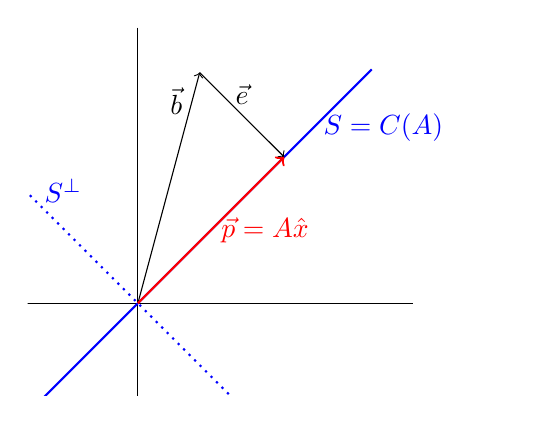
\begin{tikzpicture}[scale=2.333]
	\clip (-0.6, -0.5) rectangle (2.0, 1.5);
	 \path (-0.6, -0.5) rectangle (2.0, 1.5); % Explicit bounding box
	\draw (-1.5, 0) -- (1.5, 0);    
	\draw (0, 1.5) -- (0, -1.5);
	\draw [thick, blue] (45:-1.8cm) -- node[very near end, anchor=west] {$S=C(A)$} (45:1.8cm);
	\draw [thick, dotted, blue] (-45:-1.0cm) -- node[near start, anchor=south, yshift=2mm] {$S^{\perp}$} (-45:0.7cm);
	\draw [->] (0, 0) -- node[very near end, anchor=east] {$\vec{b}$} (75: 1.3cm);
	\coordinate (t) at (intersection of 75:1.3cm -- ++ 15:1.3cm and 0,0--45:2cm);
	\draw [->] (75:1.3cm) -- node[midway, anchor=south] {$\vec{e}$} (t);
	\draw [thick, red, -> ] (0,0)-- node[midway, anchor=west] {$\vec{p} = A \hat{x}$} (t);	
\end{tikzpicture}
\end{wrapfigure}

\parshape If we imagine some $n$-dimensional subspace $S \subseteq \R^{n}$, we can define a vector $\mathbf{b}$ that exists outside the subspace. We can also define a vector $\mathbf{p}$, the orthogonal projection of $\mathbf{b}$ onto $S$. Here we could say 
$$\mathbf{b} = \underbrace{\mathbf{p}}_{\in S} + \underbrace{\mathbf{e}}_{\in S^{\perp}} = P \mathbf{b} + (I -P) \mathbf{b}$$
For our ``projection matrix'' $P$. Now, let's imagine we define $S= C(A)$ such that $S^{\perp}= N(A^{T})$. Then, $\mathbf{p} = A \hat{x} \in C(A)$, and $\hat{x}$ is the closeset solution to $\mathbf{b}$. Therefore, $\mathbf{e} = \mathbf{b} - A\hat{x} \in N(A^{T}) \to A^{T} (b-A\hat{x}) \to A^{T}b = A^{T}A\hat{x}$. From this, we can define three \textbf{normal equations}. 
\begin{equation*}
\boxed{
\begin{align*}
			\hat{x} &= (A^{T}A)^{-1}A^{T}b \\
			\mathbf{p} &= A \hat{x} = P \mathbf{b} \\
			P &= A(A^{T}A)^{-1}A^{T}
	\end{align*}}
\end{equation*}
\begin{itemize}
	\item We can also define a handful of neat properties about the projection matrix $P$.
		\begin{enumerate}
			\item $P^{2} = P \hspace{2cm} \text{Proof.  } A(A^{T}A)^{-1}(A^{T}A)(A^{T}A)^{-1}A^{T} = P$
			\item $P^{T} = P \hspace{2cm} \text{Proof.  } \qty((A^{T}A)^{-1}A^{T}b)^{T} = (A^{T})^{T} \qty((A^{T}A)^{-1})^{T} A^{T} = P$
			\item $C(P)= C(A)$
			\item $N(P)= C(A)^{\perp} = N(A^{T})$
			\item $I-P$ is the projection matrix onto $N(A^{T})$

		\end{enumerate}
	\item Our projection vector $\mathbf{p}$ is going to minimize the norm $\|b-Ax\|$ as should be clear in the geometry above. Notably, it won't necessarily come upwith an \textit{exact solution}. Rather it is able to find the closest solution when there is no absolute solution. This is the beginning of our forees into optimization. As an example, let's examine the simplest optimization problem: least squares.
\end{itemize}

\begin{examplebox}
		\begin{wrapfigure}{l}{0.4\textwidth}
		\includegraphics[width=\linewidth]{figs/linreg.png}
		\footnotesize \centering Figure from \href{https://github.com/mitmath/18065/blob/main/notes/Least-Square%20Fitting.ipynb}{Prof. Johnson's Outstanding 18.065 Notes}
    \end{wrapfigure}
	\nident Given a time series of temperature data, we want to calculate the linear regression with our matrix methods. We are going to construct another Vandermonde matrix: this time with a highly overdetermined system. 
	$$\begin{bmatrix}
	  1 & y_1 - y_0\\
	1 & y_2 - y_0\\
	\vdots & \vdots\\
	1 & y_m - y_0
	\end{bmatrix}\begin{bmatrix}
	  x_1 \\
	x_2
	\end{bmatrix}
	= \begin{bmatrix}
	  \Delta T_1\\
	\Delta T_2\\
	\vdots\\
	\Delta T_m
	\end{bmatrix}$$

	To find our solution, we must simply minimize the orthogonal projection with the normal equations
	$$\displaystyle \argmin_{x \in \R^{2}} \|b-Ax\| = (A^{T}A)^{-1}A^{T}b$$
\end{examplebox}
	\vspace{0.5cm}
\subsection{Factorization}
\item Before we get to factorization, we should define some simple concepts that have already appeared. For instance, the \textbf{rank} of a matrix is simply the number of pivots. Simply, $\operatorname{rank} A = \dim C(A) = \dim C(A^{T})$, which should be intuitive. We can also define the \textbf{rank-nullity theorem} as $\dim N(A) = n-r$ for $r$ pivots and $n$ columns. Although we do not yet have the tools to introduce them all now, in this document we will examine \textbf{four critical factorizations}
	\begin{align}
		A &= LU \\
		A &= QR \\
		A &= U \Sigma V^{T} \\
		S &= Q \Lambda Q^{T} 
	\end{align}
	\subsubsection*{LU Factorization}
\item It turns out that matricies can be described in many ways. Some of these ways can help you solve difficult problems. The first of these is the $\bm{LU}$\textbf{-factorization}, which relates $A$ to its upper-triangular form $U$. In the process, it tells us about the inverse of a matrix. 
\item The crux of the factorization is just Gaussian elimiation of $A \leadsto U$, but storing the coefficients of each row operation in a left-multipliying matrix $L$ 
\begin{align}
	A &= \begin{bmatrix} \color{blue}{1} & 2 & 0 \\ 2 & 5 & 1 \\ -3 & 1 & -1 \end{bmatrix} \stackrel{r_2 - \color{red}{2}r_1}{\stackrel{r_3 + {\color{red}{3}}r_1}{\longrightarrow}}
    \begin{bmatrix} \color{blue}{1} & 2 & 0 \\ 0 & \color{blue}{1} & 1 \\  0 & 7 & -1 \end{bmatrix} \stackrel{r_3 - \color{red}{7}r_2}{\longrightarrow}
    \begin{bmatrix} \color{blue}{1} & 2 & 0 \\ 0 & \color{blue}{1} & 1 \\  0 & 0 & \color{blue}{-8} \end{bmatrix} = U  \\
	\implies L &= \begin{bmatrix} 1 & & \\ \color{red}{+2} & 1 & \\ \color{red}{-3} & \color{red}{+7} & 1 \end{bmatrix}
	\longrightarrow A = LU
\end{align} 
\item And as it turns out it is \textit{much} easier to calculate the inverse of a triangular matrix than a dense matrix. We can rely on $A^{-1} = (LU)^{-1} = U^{-1}L^{-1}$, and then on the kind fact that we can find each of those inverses through back substitution of $U$ and forward-substitution of $L$.
\item In reality, it's worth noting that it's not \textit{really} $A=LU$, but rather $PA=LU$. We must apply a permutation matrix to $A$ in order to account for the fact that the pivots of $A$ may not be perfectly ordered. We may at some point be forced to do a row swap, and hence apply a permutation at the end of the computation.

\subsubsection*{CR Factorization}
\item This is not one of our ``critical factorizations''. However, it is useful for us. We learned a moment ago how to compute a basis for $C(A)$. We can use that to write $A = CR$, where $C \in \R^{m \times r}$ consists of \textit{any} basis for $C$. The truth of this should be intuitive by how we have constructed the principle of a columnspace. We can take for example
	$$A = \begin{bmatrix}
	  1 & 2 & 3 & 1\\
	1 & 2 & 5 & -3\\
	1 & 2 & 7 & -7
	\end{bmatrix} \leadsto U= \begin{bmatrix}
	  1 & 2 & 0 & 7\\
	 &  & 1 & 2\\
	 &  &  & 
	\end{bmatrix}$$
	where clearly $\mathbf{c}_{1}$ and $\mathbf{c}_{3}$ are the pivot rows such that $C(A) = \span \{\mathbf{c_{1}}, \mathbf{c}_{3}\}$. We can from this express a \textit{specific case} of CR-Factorization as
	$$A = \underbrace{ \begin{bmatrix}
	  1 & 3\\
	1 & 5\\
	1 & 7
\end{bmatrix}}_C \underbrace{ \begin{bmatrix}
	  1 & 2 & 0 & 7\\
	0 & 0 & 1 & 2
\end{bmatrix}}_R$$
where, here, $C$ is the \textit{specific} column space basis corresponding to the pivot columns of the original matrix, and $R$ is the reduced row eschelon form of $A$, ommiting the trivial last row. This does not generalize to all solutions for the factorization.

	\subsubsection{QR Factorization}
	\begin{itemize}
		\item As we showed earlier, our first basis is rarely a good choice. In order to solve for any solutions we need to do a full elimination. An orthonormal basis is the cleanest basis. But how can we go from our first basis $C(A) = \begin{bmatrix}
		  \mathbf{a_{1}} & \cdots & \mathbf{a_{n}}
		\end{bmatrix} \longrightarrow \begin{bmatrix}
		  \mathbf{q}_{1} & \cdots & \mathbf{q}_{n}
		\end{bmatrix} = Q$? We can use an algorithm relying on the projection techniques above called \textbf{Gram-Schmidt} orthogonalization.
	\item We define our first orthonormal vector with respect to the first normalized first basis vector $\mathbf{q}_{1} = \dfrac{a_{1}}{\|a_{1}\|}$. From this, $\mathbf{q}_{2} = \dfrac{\overbrace{(I - \mathbf{q}_{1} \mathbf{q}_{1}^{T})}^{\operatorname{proj}_{\perp}q_{1}}\mathbf{a}_{2}}{\| \ " \ \|} = \dfrac{\mathbf{a}_{2} - \mathbf{q}_{1}(\mathbf{q}_{1}^{T}\mathbf{a}_{2})}{\| \ " \ \|}$. This pattern continues $\mathbf{q}_{3} = \displaystyle \frac{\mathbf{a}_{3} - \mathbf{q}_{1}(\mathbf{q}_{1}^{T} \mathbf{a}_{3}) - \mathbf{q}_{2}(\mathbf{q}_{2}^{T}\mathbf{a}_{3})}{\| \ " \ \|}$.  The denominator is just the norm of the numerator. This gives us a number of orthonormal vectors, but we currently have no way to actually express $A$ in terms of these vectors. We will have to work backwards.
		\begin{align*}
			\mathbf{q}_{1} &= \frac{\mathbf{a}_{1}}{\underbrace{\|a_{1}\|}_{r_{11}}} & \mathbf{a}_{1} &= \mathbf{q}_{1}r_{11} \\
			\mathbf{q}_{2} &= \frac{\mathbf{a}_{2} - \mathbf{q}_{1} \overbrace{\mathbf{q}_{1}^{T}\mathbf{a}_{2}}^{r_{12}}}{\underbrace{\| \ " \ \|}_{r_{22}}} & \mathbf{a}_{2} &= \mathbf{q}_{1}r_{12} + \mathbf{q}_{2} r_{22} \\
			\mathbf{q}_{3} &= \frac{\mathbf{a}_{3} - \mathbf{q}_{1} \overbrace{q_{1}^{T}\mathbf{a}_{3}}^{r_{13}} - \mathbf{q}_{2} \overbrace{\mathbf{q}_{2}^{T}\mathbf{a}_{3}}^{r_{23}}}{\underbrace{\| \ " \ \|}_{r_{33}}} & \mathbf{a}_{3} &= \mathbf{q}_{1}r_{13} + \mathbf{q}_{2}r_{23} + \mathbf{q}_{3}r_{33}
		\end{align*}
		and the pattern so continues, giving us 
		$$\underbrace{\begin{bmatrix}
		  \vertbar & \vertbar & \vertbar \\
		\mathbf{a}_{1} & \mathbf{a}_{2} & \mathbf{a}_{3}\\
		\vertbar & \vertbar & \vertbar
		\end{bmatrix}}_{\substack{A \\ m \times n$}}= \underbrace{\begin{bmatrix}
  \vertbar & \vertbar & \vertbar\\
\mathbf{q}_{1} & \mathbf{q}_{2} & \mathbf{q}_{3} \\
\vertbar & \vertbar & \vertbar
\end{bmatrix}}_{\substack{Q \\ m \times n}} \underbrace{\begin{bmatrix}
  r_{11} & r_{12} & r_{13}\\
 & r_{22} & r_{23}\\
 &  & r_{33}
\end{bmatrix}}_{\substack{R \\ n \times n}}$$
\item It is assumed here that $A$ is \textbf{full column rank}. Hence, it will either be square or ``tall''. $R$ is upper-triangular and invertible. $R$ is upper triangular because, as we saw in the Gram-Schmidt algortihm, we construct our basis columns $\mathbf{q}_{i}$ of $Q$ in the first place based on only $\mathbf{a}_{j \leq i}$
\item For the purposes of 18.C06 as a class, it is much more important to understand the \textit{shapes} and \textit{behavior} of this factorization than work through the computation of the basis and $R$ itself. THe full equations earlier were mostly expressed long-form to give a sense of the pattern how this relates to the projections into each orthogonal vector.

\subsubsection{Singular Value Decomposition}
\item Ah, finally. The ``factorization to rule them all'', the \textbf{SVD}, which holds the deepest insight we can gain into the behavior of a matrix from it's representation in the four essential subspaces. For a rank-$r$ matrix $A \in \R^{m \times n}$, we express it in it's ``compact form'' as

		$$A = \underbrace{\begin{bmatrix}
		  u_1 & u_2 & \cdots & u_r
  \end{bmatrix}}_{\text{orthonormal basis for }C(A)} 
  \underbrace{\begin{bmatrix}
\sigma_1 &  & \\
   & \ddots & \\
   &  & \sigma_r
\end{bmatrix}}_{\text{scale factors } \sigma_k > 0}
\underbrace{
\begin{bmatrix}
  v_1 & v_2 & \cdots & v_r
\end{bmatrix}^T
}_{\text{orthonormal basis for }C(A^T)} = \hat{U} \hat{\Sigma} \hat{V}^T$$
\item We call the vectors constituting matrix $\hat{U}$ the \textbf{left-singular} vectors, the vectors of $\hat{V}^{T}$, the \textbf{right-singular} vectors, and the scalar constants of $\hat{\Sigma}$ the \textbf{singular values}. These singular values are in sorted order, from greatest to smallest. This is essential.
\item In general, it is very difficult to compute this factorization. For now we just won't worry about it. Furthermore, we won't worry \textit{why} it exists either until we discuss eigenvalues and eigenvectors.
\item So how does this work? Let's consider it's mathematical ``mechanism of action'' so to speak.
	\begin{enumerate}
		\item $Ax \to U\Sigma (V^{T} x)$. This first projects $x$ onto $C(A^{T})$. If we recall the geometry of our fundemental subspaces,we see that this operation will project $x$ orthogonal to $N(A)$, which is desirable. 
		\item In $C(A^{T})$, we scale up the components of $\hat{V}^{T}x$ using our singular-value matrix $\hat{\Sigma}$. This gives us our desired magnitudes. 
		\item We project into our final $C(A)$ using $\hat{U}$ to give our final vector $Ax$
	\end{enumerate}
\item If we look at our expression for the SVD earlier, it might appear how we cold express it in terms of a summation. For rank-$r$ matrix $A$, consider
	$$A = \hat{U}\hat{\Sigma} \hat{V}^{T} = \sum_{i=1}^{r}\sigma_{i}u_{i}v^{T}_{i}$$
\item Imagine that we do not take the sum to completion. Instead, we only consider the first terms $k \leq r$. If we recall that the singular values are in sorted order, the \textbf{Eckart-Young Theorem} tells us that the best approximation for $A$ of rank $k$ is $A \approx \displaystyle \sum_{i=1}^{k}\sigma_{i}u_{i}v_{i}^{T}$. The output of this is called the \textbf{truncated SVD}.
\item If we consider the shapes of our matricies $\hat{U}\hat{\Sigma} \hat{V}^{T}$, we see that $\hat{U},\ \hat{V}^{T}$ are very rarely square. This means that they cannot be invertible, which could be inconvienent. In order to solve this, let's construct the \textbf{full SVD}. Currently the columns of $\hat{U}$ are an orthonormal basis for $C(A)$. Let's append a basis of $N(A^{T})$ such that $U = \begin{bmatrix}
  U_{r} & U_{\perp}
\end{bmatrix}$, and a basis of $N(A)$ to $V$ such that $V = \begin{bmatrix}
  V_{r} & V_{\perp}. 
\end{bmatrix}$. We don't actually want any component of these vectors in our output, so we will modify $\hat{\Sigma}$ with the appropriate shape to 0 the components in the complementary spaces.
$$A = \underbrace{\begin{bmatrix}
  u_{r} & \cdots & u_{m}
  \end{bmatrix}}_{\substack{U \\ m \times m}} \underbrace{\begin{bmatrix}
  \sigma_{1} &  &  &  & \\
 & \ddots &  &  & \\
 &  & \sigma_{r} & 0 & \cdots\\
 &  & 0 & 0 & \cdots \\
 &  & \vdots & \vdots & \ddots
\end{bmatrix}}_{\substack{\Sigma \\  m \times n}} \underbrace{\begin{bmatrix}
  v_{1} & \cdots & v_{n}
\end{bmatrix}^{T}}_{\substack{V^{T} \\ n \times n} $$
for $\Sigma$ with $n-r$ extra columns of 0's and $m-r$ extra rows of 0's compared to $\hat{\Sigma}$.
\end{itemize}

\begin{ideabox}[Norms and Transformations]
	\begin{wrapfigure}{l}{0.42\textwidth}
	    \includegraphics[width=0.4\textwidth]{figs/ellipse.png}

		\footnotesize \centering Figure from \href{https://nbviewer.org/github/mitmath/1806/blob/fall22/notes/SVD-intro.ipynb}{Prof. Johnson's 18.C06 Notebooks}
	\end{wrapfigure}
	\ndent A useful way to think of linear transformations on an orthonormal basis is an operator that transforms a unit circle into an ellipsoid, as the figure shows. This visualization is also the key to connecting the SVD to the eigenvectors of a matrix, which is perhaps the deepest connection in all of linear algebra. 
	\\\\
\noindent We also can define here the \textbf{operator norm}, which is the largest amount by which $A$ can stretch its orthonormal basis. For our case of SVD, the operator norm is always just the largest singular value. \\ \\
\noindent This leads naturally to our formal definition of a \textbf{norm}. 
	Given a vector space $V$ a \textbf{norm} is a map $\vec{v} \in V \mapsto \|\vec{v}\| \elem \mathbb{R}$ satisfying
	\begin{enumerate}
		\item	\textbf{Non-negative: }$ \|\vec{v}\| \geq 0$. ($=0$ iff $\vec{v}=\vec{0}$) 
		\item \textbf{Scaling: }$ \|\alpha \vec{v}\| = \alpha \|\vec{v}\|$
		\item \textbf{Triangle Inequality: } $\|\vec{v_1} + \vec{v_2}\| \leq \|\vec{v_1}\| + \|\vec{v_2}\|$
	\end{enumerate}
\end{ideabox}
\begin{examplebox}[1.7]\quad
	\noindent Using this definition let's prove our lemma about the operator norm
	$$\|Ax\|_0 = \displaystyle \max_{x \in \R^{n}} \frac{\|Ax\|}{\|x\|} = \sigma_{\texttt{max}}$$. 
	\begin{solution}[1.7]\quad
		\begin{enumerate}
			\item First let's first prove $\|Ax \| \geq 0$. $\|Ax\| = (Ax)^{T}(Ax) = x^{T}A^{T}A^{T} = x^{T}V\Sigma U^{T}U \Sigma V^{T}x = v^{T}V \Sigma^{2}V^{T}x = (V^{T}x)^{T}\Sigma^{2}(V^{T}x)$. Let's define $c = V^{T}x$. Then, we can decompose the system down to a sum of vector dot products such that $c^{T}\Sigma^{2}c = \displaystyle\sum_{i=1}^{r}\sigma_{i}^{2}c_{i}^{2}$.
			\item By the triangle equality, $\|x \| \geq \| V V^{T} x\|$ since $VV^{T}$ is just a projection matrix that cannot increase the norm of $x$. From this we can  say $\|V V^{T}x\| = (VV^{T}x)^{T}(VV^{T}x) = x^{T}VV^{T}VV^{T}x = x^{T}VV^{T}x = (V^{T}x)^{T}(V^{T}x)$ which, by the $c$ we defined earlier equals $c^{T}c$. If we express it simarly as a sum, $\|x \| \geq c^{T}c = \displaystyle\sum_{j=1}^{r}c_{j}^{2}$.
			\item Putting the last two steps together, $\displaystyle \frac{\|Ax\|}{\|x\|} = \sqrt{ \frac{\sum \sigma_{i}^{2}c_{i}^{2}}{\sum c_{i}^{2}} } = \sqrt{\sigma_{\texttt{max}}^{2}} = \sigma_{\texttt{max}}$ 
		\end{enumerate}
	    
	\end{solution}
	\begin{takeaways}[1.7]\quad
		\begin{itemize}
			\item The decomposition of $\Sigma$ into the sum of singular values is a very tricky lifesaver. 
			\item You can get a lot out of expressing the 2-norm in terms of $x^{T}x$. Things often cancel which will lead you with an interesting expression.
		\end{itemize}
	    
	\end{takeaways}
\end{examplebox}
\begin{itemize}
	\item So why is any of that useful? Let's take a look at \textbf{error propogation} when solving linear systems. Suppose $\text{shape } A = m \times m$, $\rank A = r$ and $x = A^{-1}b.$ If we make a little error $\Delta b$ in $b$ (roundoff error, measurement noise, &c), what is the error $\Delta x$? 
		$$A^{-1}(b + \Delta b) = A^{-1}b + A^{-1}\Delta b = x + \Delta x$$
This equation really doesn't tell us much. We want to know how $\Delta b$ scales with $\|b\|$ and how $\Delta x$ scales with $\| x\|$.
$$\frac{\| \Delta b \|}{\| b \|} = \frac{\| Ax \|}{\| x \|} \frac{\| \Delta x\|}{\|\Delta b\|} \leq \| A \| \| A^{-1}\| = \frac{\sigma_{\texttt{MAX}}}{\sigma_{\texttt{MIN}}} \equiv K(A)$$
where we are defining $K(A)$ as the \textbf{condition number} of $A$. This tells us how close $A$ is to being singular.
	\item For example, the least singular matrix is $I$. $A = U \Sigma V^T = I I I $. All $\sigma=1$. $K(I) = 1$. This also applies for any orthogonal matrix or multiple of $Q$ or $I$.
\end{itemize}
		\begin{ideabox}[Penrose Pseudo-inverse]\quad\\
			With the SVD factorization, we can also describe the \textbf{pseudo-inverse} $A^{+}$ of $A$. This is a contrived generalization on our established idea of a matrix inverse that allows non-square matricies to be ``inverted'' such that $A^{+}A = I \ \forall \ A \in \R^{m \times n}$.
			$$A^+ = \hat{V}\hat{\Sigma}^{-1}\hat{U}^T = \begin{cases}
			A^{-1} &\text{if } m=n \text{ (square)} \\
			(A^T A)^{-1}A^T &\text{if } n=r \text{ (tall)} \\
			A^T(A A^T)^{-1} &\text{if } m=r \text{ (wide)} \\
		\end{cases}$$
		    
		\end{ideabox}
\begin{examplebox}[1.8]\quad\\
	\noindent Prove using SVD that $A^{T}A$ is invertible if $A$ has full column rank and $C(A^{T}A) = C(A^{T})$.\vspace{0.14cm}
\begin{solution}[1.8]\quad\\
	Say $A \in \R^{m \times n}$ and $\operatorname{rank} A = r$ so that $A = \hat{U} \hat{\Sigma} \hat{V}^{T} \to A^{T}A = \hat{V}\hat{\Sigma}\hat{U}^{T}\hat{U} \hat{\Sigma} \hat{V}^{T} = \hat{V}_{n \times r}\hat{\Sigma}^{2}_{r \times r}\hat{V}^{T}_{r \times n}$. Since $A$ is full column-rank, $n=r$ and $\operatorname{rank} A^{T}A=n$. Knowing $A^{T}= \hat{V} \hat{\Sigma} \hat{U}^{T}$, we see that $\hat{V}$ spans $C(A^{T})$. We see the same in $A^{T}A = \hat{V} \hat{\Sigma^{2}}\hat{V}^{T}$ showing that $C(A^{T}A) = C(A)$    
\end{solution}
\begin{takeaways}[1.8]\quad
    \begin{itemize}
		\item The SVD transforms the vector into the column space spanned by the first matrix. This isn't always an obvious subspace.
		\item Consider writing out the shapes of the matricies explicitly during algebra.
    \end{itemize}
\end{takeaways}
\end{examplebox}
\subsection{Eigenproblems}
\begin{itemize}
	\item We have finally arrived at the biggest idea in linear algebra: eigenvalues and eigenvectors. These eigenproblems, so called, are the web with which we can tie together almost everything in linear algebra. They will also lead us to our final factorization $S = Q \Lambda Q^{T}$. For now, unfortunately, I must be coy, and insist we visit the determinant. 
		\subsubsection*{Determinant}
	\item You may be surprised the determinant has not been so far mentioned. In reality, it's just not that useful for modern applications. But why don't we care about determinants anymore? While $\det A = ad-bc$ in $\R^{2}$, it turns out that past $\R^{4}$, the calculation of a determinant becomes so clumsy that we either must abstract it to computer computation or, if we are conservative about our compute, find ways to go around it to begin with.
	\item Geometrically, the determinant represnts the factor by which the area of parallelogram between two vectors is multiplied as the result of a vector a transformation. The following figure may elucidate this obscure geometric meaning.
		$$
		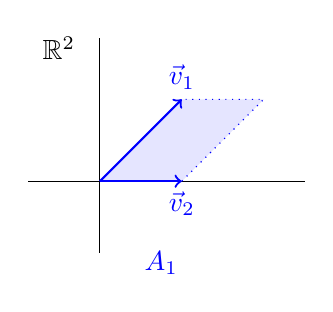
\begin{tikzpicture}[scale=1.3, baseline]
    % Input space
    \draw (-0.7, 0) -- (2, 0);
    \draw (0, -0.7) -- (0, 1.4);
    
    % Original parallelogram with fill
    \fill[blue!10] (0,0) -- (0.8,0.8) -- (1.6,0.8) -- (0.8,0) -- cycle;
    % Original vectors
    \draw[thick, blue, ->] (0,0) -- (0.8,0.8) node[above] {$\vec{v}_1$};
    \draw[thick, blue, ->] (0,0) -- (0.8,0) node[below] {$\vec{v}_2$};
    \draw[blue, dotted] (0,0) -- (0.8,0.8) -- (1.6,0.8) -- (0.8,0) -- cycle;
    \node[blue] at (0.6,-0.8) {$A_1$};
    
    % Label input space
    \node at (-0.4, 1.3) [anchor=center] {$\mathbb{R}^2$};
\end{tikzpicture}
\quad
\raisebox{0.00em}{
\xrightarrow{\qquad A = \begin{bmatrix}
  2 & 0\\
1 & 1
\end{bmatrix} \qquad}
}\quad
\quad
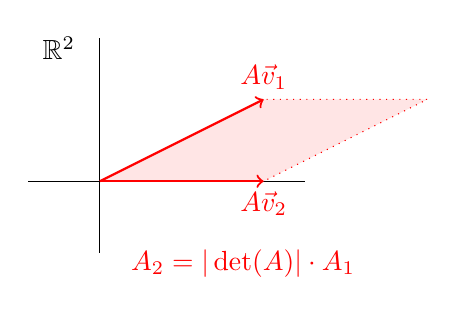
\begin{tikzpicture}[scale=1.3, baseline]
    % Output space
    \draw (-0.7, 0) -- (2, 0);
    \draw (0, -0.7) -- (0, 1.4);
    
    % Transformed parallelogram with fill
    \fill[red!10] (0,0) -- (1.6,0.8) -- (3.2,0.8) -- (1.6,0) -- cycle;
    % Transformed vectors
    \draw[thick, red, ->] (0,0) -- (1.6,0.8) node[above] {$A\vec{v}_1$};
    \draw[thick, red, ->] (0,0) -- (1.6,0) node[below] {$A\vec{v}_2$};
    \draw[red, dotted] (0,0) -- (1.6,0.8) -- (3.2,0.8) -- (1.6,0) -- cycle;
    \node[red] at (1.4,-0.8) {$A_2 = |\det(A)| \cdot A_1$};
    
    % Label output space
    \node at (-0.4, 1.3) [anchor=center] {$\mathbb{R}^2$};
    
    % Matrix definition
\end{tikzpicture}
$$
\item Yet, we are not geometers here. The most cherished property of the determinant is its part in deriving the eigenvalues and vectors. For that, we must understand its algebra. Symbolically, we can name many determinant identities that are useful. Here is a curation.
	\begin{enumerate}
		\item \textbf{Zeros:} $\det A = 0$ if $A$ is singular.
		\item \textbf{Normalization: }$\det I = 1$.
		\item \textbf{Swaps: } If you switch rows of $A$, flip the sign of $\det A$.
		\item \textbf{Multiplication: }$\det(AB) = \det A \det B$
		\item \textbf{Inverse: }$\det A^{-1} = \frac{1}{\det A}$
		\item \textbf{Transpose: }$\det A^{T} = \det A$
		\item \textbf{Linearity: }$\det \mtwtw{\alpha a}{\alpha b}{c}{d} = \alpha \det \mtwtw{a}{b}{c}{d} \longrightarrow \det (\alpha A) = \alpha^{n} \det A$ for $A \in \R^{n \times n}$.
	\item \textbf{Row operations: }Adding a multiple of one row $\alpha r_{i}$ to another $r_{k}$ does not affect the determinant. \textit{Note this does \textit{not} imply that $\det A$ is invariant under row operations (i.e. permutation, scalar multiplication, \&c)}.
	\item \textbf{Triangular matricies: }For upper triangular matrix $U = \begin{bmatrix}
	  d_{1} & * & *\\
	 & d_{2} & *\\
	 &  & \ddots
	\end{bmatrix}$, $\det U = \displaystyle \prod_{i=1}^{k}d_{i}$.
	\end{enumerate}

	\subsubsection*{Eigenvalues}
\item The central idea of eigenvalues and eigenvectors is that we can find some vectors for which a linear operator $A$ acts like a scalar multiplier $\lambda$ on $x$. That is, only the \textit{magnitude} of $x$ is affected. It's direction stays the same. We express this as
$$\boxed{Ax = \lambda x}$$
When this is true, we say $x$ is our \textbf{eigenvector}, and $\lambda$ is our \textbf{eigenvalue.}
\item Normally, for a matrix $A \in \R^{n \times n}$, we will find $n$ corresponding eigenvalues and eigenvectors $\lambda_{1},\ \lambda_{2},\ \ldots \ , \lambda_{n}$. A matrix that satisfiees this condition is called \textbf{diagonalizable}. Very few matricies will not. And we will address their special case, called ``defective matricies'' in due time.
\item We will try to construct a basis of eigenvectors $X$ such that we can take any vector $x$ and expand it in the basis $x = c_{1}x_{1} + c_{2}x_{2} + \cdots = Xc$. For each eigenvector $x_{k}$, $A$ acts as the scalar $\lambda_{k}$. In order to find the vectors, we much find the eigenvalues. 
\end{itemize}

\end{itemize}


\begin{wrapfigure}{l}{0.4\textwidth}
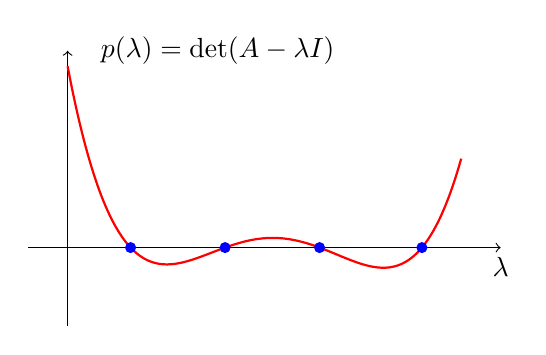
\begin{tikzpicture}
    % Axes
    \draw[->] (-0.5, 0) -- (5.5, 0) node[anchor=north] {$\lambda$};
    \draw[->] (0, -1) -- (0, 2.5) node[anchor=west, xshift=3mm] {$p(\lambda) = \det(A - \lambda I)$};

    % Quartic polynomial (degree-4)
    \draw[red, thick, smooth, samples=100, domain=0:5] 
        plot (\x, {0.1*(\x-0.8)*(\x-2)*(\x-3.2)*(\x-4.5)});

    % Roots (eigenvalues)
    \foreach \x in {0.8, 2, 3.2, 4.5} {
        \fill[blue] (\x, 0) circle (2pt);
    }

    % Dotted line for x-axis
\end{tikzpicture}
\end{wrapfigure}
\noindent \hspace{-0.5cm} \textbullet \ \ Our defining case $Ax = \lambda_{k} x \implies (A - \lambda_{k} I)x = 0$, meaning that for $\lambda_{k}$, $A - \lambda_{k}I$ is singular, or $p(\lambda) = \det (A - \lambda_{k}I) = 0$. Our determinant will expand into some \textbf{characteristic polynomial} $p(\lambda)$. If $A$ is square, the roots of $p(\lambda)$ are the eigenvalues. For example if we have
$$A = \mtwtw{1}{1}{-2}{4}$$
It's eigenvalues can be calculated by simply
\begin{align*}
	\det (A - \lambda I) = \det \begin{bmatrix}
     1 - \lambda & 1\\
   -2 & 4 - \lambda
\end{bmatrix} 
&= (1 - \lambda)(4-\lambda) - (1)(-2)\\ &= \lambda^{2}-5\lambda + 6 = (\lambda -2)(\lambda - 3) \\
&\implies \lambda_{1,2} = \{2,\ 3\}.
\end{align*}
\begin{itemize}
	\item Since we are dealing with polynomials here, we must prepare for our eigenvalues to be complex. In the case we have $\lambda_{i} \in \mathbb{C}$ for a real matrix, the complex eigenvalues will form a \textbf{complex conjugage pair}. We will see this again soon.
\subsubsection*{Eigenvectors}
    \item Once we have the eigenvalues, the eigenvectors are just a basis for the $N(A - \lambda I)$. In our case from above
		\begin{align*}
			A - 2I = \mtwtw{-1}{1}{-2}{2} \text{ such that } (A - 2I)x_{1} = \mtwtw{-1}{1}{-2}{2} \vtwoC{1}{1} = \vtwoC{0}{0}
		\end{align*}
		revealing that $x_{1} = \vtwoC{1}{1}$. We repeat the same operation for $\lambda_{2} = 3$ to discover $x_{2} = \vtwoC{1}{2}$.

\subsubsection*{Diagonalization}
\item So why have we done all this to begin with? Really the purpose of constructing this eigenvector basis is to give us much greatear flexibility with our matrix operations. For an arbitrary matrix $A$, taking $A^{4}$ is a nightmare by naive methods. We can use our eigensolutions to give us a much deeper insight into these kinds of problems. For example, using our same $A$ as above,
	$$A^{n}\vtwoC{2}{3} = A^{n} \bigg(\underbrace{\vtwoC{1}{1} + \vtwoC{1}{2}}_{x_{1}+x_{2}}\bigg) = 2^{n} \vtwoC{1}{2} + 3^{n} \vtwoC{1}{2} \approx 3^{n} \vtwoC{1}{2} \text{ for } n \gg 1$$
	as $n$ grows, the largest eigenvector will \textbf{dominate} all smaller terms.
\item This is a pretty slick expression. However you may be skeptical about how contrived the vector $\begin{bmatrix}
  2 & 3
\end{bmatrix}^{T}$ is. Recalling diagonalization above, we can generalize this into a marvelous form. Recall, we are generally doing all of this to construct a basis of eigenvectors $X$. With this we can say something like

\begin{align*}
	AX = \begin{bmatrix}
  Ax_{1} & Ax_{2} & \cdots & Ax_{n}
  \end{bmatrix} &= \begin{bmatrix}
  \lambda_{1}x_{1} & \lambda_{2}x_{2} & \cdots & \lambda_{n}x_{n}
\end{bmatrix}\\
&= X \begin{bmatrix}
  \lambda_{1} &  & \\
 & \ddots & \\
 &  & \lambda_{n}
\end{bmatrix}= X \Lambda \\
	\Aboxed{A \vec{y} &= X \Lambda X^{-1} \vec{y}}
\end{align*}
\begin{itemize}
	\item $\bm{X^{-1}}\mathbf{y} \equiv \mathbf{c}$ projects $y$ into the $X$ basis.
	\item $\bm{\Lambda}$ multiplies each coefficient $c_{k}$ by it's appropriate $\lambda_{k}$.
	\item $\bm{X}$ adds up the eigenvectors and their coefficients.
\end{itemize}
\item With this, we can now make useful expressions such as $\vec{y} = \vec{x}_{1}c_{1} + \vec{x}_{2}c_{2}+ \cdots$ or similarly that $A \vec{y} = \lambda_{1}\vec{x}_{1}c_{1} + \cdots$.
\item Now why did we expend all of that effort? We can connect this to our example of matrix powers above in a \textit{much} more elegant way. Here,  $A^{n} = X\Lambda X^{-1}X \Lambda X^{-1}X\Lambda X^{-1}\cdots = \boxed{X\Lambda^{n} X^{-1}}$. Since $\Lambda$ is a diagonal matrix, $\Lambda^{n} = \operatorname{diag} \qty(\lambda_{1}^{n},\ \lambda_{2}^{n}, \ \cdots \ \lambda_{r}^{n})$ which is just scalar multiplication.
\item And, as we saw earlier with eigenvalue domination, for large $n$,
	$$\Lambda^n  = \lambda_{1}^{n}\begin{bmatrix}
	  1 &  & \\
	 & (\lambda_{2}/\lambda_{1})^{n} & \\
	 &  & \ddots
	\end{bmatrix} \approx \begin{bmatrix}
	  1 &  & \\
	 & 0 & \\
	 &  & \ddots
	\end{bmatrix}$$ 
	as the lower-order terms get exponentially small.
	\\
	\begin{ideabox}[Determinant and Trace]
	    Before going any further, let's quickly define two facts that we will exploit thoroughly. We define the \textbf{trace} operation $\trace A$ as the sum of it's diagonal enteries for any square $A$. It obeys a handful of nice properties, particularly that $\trace (AB) = \trace (BA)$. Therefore, $\trace A = \trace (X \Lambda X^{-1}) = \trace ( X X^{-1} \Lambda) = \trace \Lambda$. Simply put,
		$$\trace A = \sum_i \lambda_i$$
		We can also uncover a hideen identity of the determinant now. As we established earlier, $\det (AB) = \det A \det B$. Therefore $\det A = \det X \det \Lambda (\det X)^{-1} = \det \Lambda$. Alternatively,
		$$\det A = \prod_i \lambda_i$$
		These results are \textit{very} useful. Last but not least, these operations also define a shortcut formula for our characteristic polynomial $$p(\lambda) = \lambda^{2} - \trace A + \det A$$
	\end{ideabox}

\item We would say that a matrix $A$ is \textbf{similar} to $B$ if $A = SBS^{-1}$ for some invertible $S$. Should this be true we can say $\det A = \det B,\ \trace A = \trace B,\ \det (A - \lambda I) = \det (SBS^{-1} - \lambda SS^{-1}) = \det (S (B- \lambda I)S^{-1}) = \det(B- \lambda I)$. In short, the eigenvalues are the same, but the eigenvectors are not.

\end{itemize}

\section{Applied Linear Algebra}
\subsection{Tikhonov Regularization}
\subsection{Statistics}

\begin{itemize}
	\item For some black box distribution that generates samples $x_k$, we have $m$ data points and sample mean 
		$$\mu = \frac{1}{m}\sum_{k=1}^{m}x_{k}.$$
	As the limit $m\to \infty$ the sample mean $\mu$ approach the true mean. Until then, we say the \textbf{sample variance} $S^2$
	$$\text{Var}(x) = S^2 = \frac{1}{m-1}\sum_{k=1}^{m} (x_{k}-\mu)^{2}$$
\item We can define the statistical mean in linear algebra terms by establishing $\vec{o} = \begin{pmatrix}
  1 & 1 & \cdots & 1
\end{pmatrix}^T$. By the definition of the dot product we know $\sum_{i=1}^{n} x_i= \vec{o}^T x$ and that $m=o^T o$. Substituting these into our summation, $\mu = \frac{o^Tx}{o^T o}$. We can rewrite the variance in a similar way
$$\text{Var}(x) = \frac{\|\vec{x} - \mu \vec{o}\|^2}{m-1} = \frac{\| (I - \frac{o o ^T}{o^T o} )\vec{x}\|^2}{m-1}$$
\item One may also be interested in evaluating the correlation between two sets of data, as measured by the \textbf{covariance}. For two variables $x$ and $y$,
	$$\text{Covar}(x, y) = \frac{1}{m-1}\sum_{k=1}^{m}(x_k - \mu_x)(y_k - \mu_{y} = \frac{(Px)^T(Py)}{m-1} = \frac{x^TPy}{m-1}$$
	for projection matrix $P = I - \frac{oo^T}{o^To}$.
\end{itemize}

\end{document}

